\documentclass[letterpaper,12pt,oneside]{book}
\usepackage[top=1in, left=1.25in, right=1.25in, bottom=1in]{geometry}
\usepackage{bachelorstitlepageUNAM}

\author{Luis Esteban Serrano Bermúdez}
\title{}
\faculty{Facultad de Ingeniería}
\degree{Ingeniero en Computación}
\supervisor{Dr. ... Tutor}
\cityandyear{Ciudad Universitaria, Cd. Mx., 2020}
\logouni{Escudo-UNAM}
\logofac{Escudo-FING}

\usepackage[T1]{fontenc}
\usepackage[utf8]{inputenc}
\usepackage[spanish,es-nodecimaldot,es-tabla]{babel}
\usepackage{graphicx}
\usepackage{subfigure}
\usepackage{tikz}
\usepackage{pdfpages}

\graphicspath{{./figs/}}
\usepackage{setspace}

\begin{document}
	\frontmatter
	\maketitle
	\chapter*{}

	\begin{flushright}
	  \emph{Dedicatoria ...} 
	  \thispagestyle{empty}
	\end{flushright}

	\chapter{Agradecimientos}
	\spacing{1.5}

	\chapter{Resumen}

	\tableofcontents
	\listoffigures
	\listoftables

	\chapter{Prólogo}
    Este proyecto se ha desarrollado con la finalidad de añadir una mejora a los medidores de energía previamente realizados en el Instituto de Ingeniería de la UNAM. La finalidad de esta mejora es agregar una función de lectura de datos de registros del medidor de energía ADE7880 para poder analizar una gran cantidad de datos en poco tiempo.

	\mainmatter

%%%%%%%%%%%%%%%%%%%%%%%%%%%%%%%%%%%%%%%%%%%%%%%%%%%%%%%%%%%%%%%%%%%%%%%%%%%%%%%
%%%%%%%%%%%%%%%%%%%%%%%%%%%%%%%%% INTRODUCCIÓN %%%%%%%%%%%%%%%%%%%%%%%%%%%%%%%%
%%%%%%%%%%%%%%%%%%%%%%%%%%%%%%%%%%%%%%%%%%%%%%%%%%%%%%%%%%%%%%%%%%%%%%%%%%%%%%%
	\chapter{Introducción}

		\section{Computadora}
		Una computadora esta conformada por hardware y software. La parte de Hardware consta de 4 componentes: el procesador, que funciona como el cerebro; la unidad de entrada, por la cual los programas y los datos son ingresados; la unidad de salida por donde son presentados los los resultados y la memoria que es en donde se almacena el software y los datos.

			\subsection{Procesador}
			El procesador, tambien llamada como la Unidad Central de Procesamiento se puede clasificar en tres partes:
		
			\begin{itemize}
				\item \textbf{Registros:} Es una locación de almacenamiento dentro de la CPU en la cual se mantienem los datos y las direcciones de memoria durante la ejecución de una instrucción. Accesar a los registros de datos es más rápido que acceder a los datos en la memoria externa. Estos registros varían dependiendo del modelo del procesador.

				\item \textbf{Unidad Lógica Aritmética:} Es la calculadora numérica y evaluadora lógica de operaciones. Aquí se reciben los datos provenientes de la memoria principal o de los registros, realiza una operación lógica y si es necesario reescribe el resultado de vuelta al registro o memoria.

				\item \textbf{Unidad de Control:} Contiene las instrucciones lógicas del hardware, esta se encarga de decodificar y monitorear la ejecución de las instrucciones. Tambien funciona como árbitro de varios de los servicios del CPU, los cuiales se encuentran sincronizados por un reloj de sistema.
			\end{itemize}

			\subsection{Arquitecturas de Procesadores}

				\subsubsection{Arquitectura Harvard}
				El término de Arquitectura Harvard se le conoce a aquellas configuraciones donde las instrucciones y los datos de entrada/salida se almacenan por separado en 2 memorias, este término se le conoce por la primer computadora digital automática el "\textit{Harvard Mark I}" (1944) diseñado por IBM y la Universidad de Harvard\cite{cuellar2008sistemas}.

				\begin{figure}[!htpb]
					\centering
					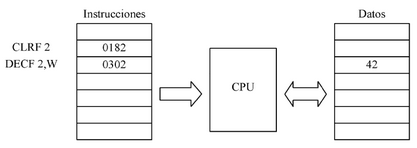
\includegraphics[scale = 1.0]{Material de Consulta/ArqHrv.PNG}
					\caption[Arquietctura Harvard]{Arquietctura Harvard}
					\label{ArqHrv}
				\end{figure}

				La arquitectura Harvard duplica efectivamente el espacio accesible de memoria y la velocidad teórica de ejecución, ya que el procesador puede realizar las operaciones de lectura y escritura sobre los 2 buses a la vez y leer datos e instrucciones en el mismo ciclo\cite{caprile2012desarrollo}.

				\subsubsection{Arquitectura Von Neumann}
				Esta arquitectura usa la misma memoria para instrucciones como para datos, es decir, utiliza una memoria de lectura/escritura para estoa procesos. En esta arquitectura no hay diferencia entre datos e instrucciones, todos son números y solo depende del uso que se le asigne. Esto ha permitido el desarrollo de procesaores simples y relativamente eficientes.

				\begin{figure}[!htpb]
					\centering
					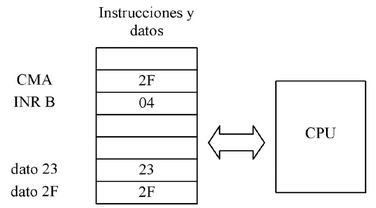
\includegraphics[scale = 1.0]{Material de Consulta/ArqVNm.PNG}
					\caption[Arquietctura Von Neumann]{Arquietctura Von Neumann}
					\label{ArqVNm}
				\end{figure}

				En estos casos es común el tener un programa para tomar datos externos, almacenarlos como datos en la memoria y ejecutarlos como instrucciones.

				Actualmente se tienen microprocesadores de ambas arquitecturas y depende de las necesidades de cada situación en la que se beneficiaá del uso de una u otra arquitectura.

				\subsubsection{Puertos}
				Los puertos son un conjunto de conexiones con las que el procesador puede interactuar con el mundo exterior a través de señales digitales.

				\begin{figure}[!htpb]
					\centering
					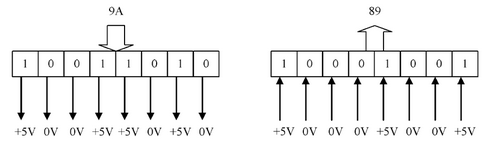
\includegraphics[scale = 1.0]{Material de Consulta/PuertosE-S.PNG}
					\caption[Puertos de Entrada y Salida]{Puertos de Entrada y Salida}
					\label{PrtsES}
				\end{figure}

				Un procesador considera a estos como locaciones de memoria que se escriben o leen datos. A un puerto que toma datos del exterior se le conoce como puertos de entrada (input) y si envía información al exterior entonces es de salida (output). Generalmente a estos puertos se les conoce como Puertos I/O.

				\begin{figure}[!htpb]
					\centering
					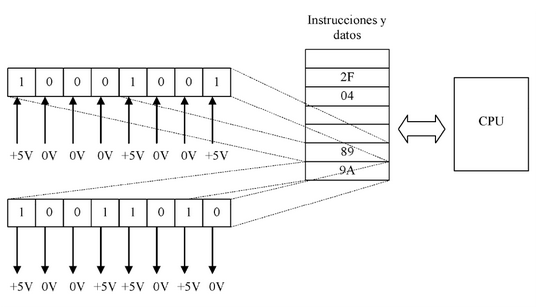
\includegraphics[scale = 1.0]{Material de Consulta/PrtsIO.PNG}
					\caption[Memoria y Puertos I/O]{Interacción de puertos con la memoria y con el procesador}
					\label{PrtsIO}
				\end{figure}

		\section{Microprocesador}
		El procesador en una computadora, esta comprendido de varios circuitos integrados, mientras que un microprocesador es un procesador empaquetado en un único circuito integrado. Una microcomputadora usa un microprocesador como su CPU\cite{valdes2007microcontroladores}.

		Los microprocesadores vienen en diferentes presentaciones, 4-Bits, 8-Bits, 16-bits, 32-Bits e incluso en 64-Bits aunque estos últimos no son demasiado comunes como los anteriores. El número de bits corresponde al número de digitos binarios que el microprocesador puede manipular en las operaciones.

		El acceso de la memoria principal toma mucho más tiempo que el tiempo de reloj disponible por el CPU, por ello es que los microprocesadores de 32 y 64 Bits poseen una textit{memoria caché} de alta velocidad.

		\section{Microcontrolador}
		Una microcomputadora se compone de 3 bloques fundamentales: CPU, Memoria y los puertos de entrada/salida. Estos se conectan entre si mediante grupos de lineas eléctricas denominados buses; los cuales pueden ser de direcciones, si transportan direcciones de memoria, o de datos, si en cambio transportan datos o instrucciones, o de control si estos conducen diversas señales de control.

		\begin{figure}[!htpb]
			\centering
			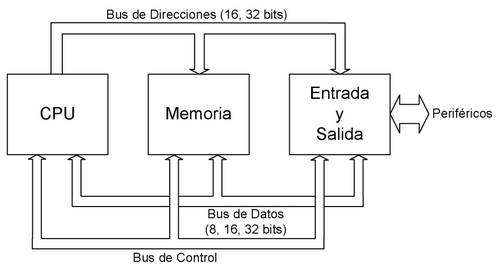
\includegraphics[scale = 1.0]{Material de Consulta/EsqMicro.PNG}
			\caption[Esquema básico general de un microprocesador]{Esquema básico general de un microprocesador}
			\label{EsqMicro}
		\end{figure}

		El CPU es el encargado en traer las instrucciones alojadas en la memoria, interpretarlas y hacer que se ejecuten. En una micromputadora la CPU es el microprocesador por lo cual un Microcontrolador es una Microcomputadora fabricada en un Circuito Integrado.

		Los microcontroladores son construidos fundamentalmente para aplicaciones puntuales en automoción, equipos de comunicaciones y telefonía, instrumentación electrónica, equipos médicos e industriales, electrodomésticos, etc. donde se deben realizar un pequeño número de tareas al menor costo posible. En estas el microcontrolador ejecuta un programa almacenado permenentemente en la memoria interactuando con datos almacenados temporalmente e interactua con el exterior a traves de las líneas de entrada/salida. El microcontrolador es parte de la aplicación(Controlador Embebido).

			\subsection{Elementos Principales}
			Además de la microcomputadora (CPU, memori y lineas de entrada/salida) los microcontroladores disponen de más componentes para poder realizar el funcionamiento requerido por las aplicaciones.

			\begin{figure}[!htpb]
				\centering
				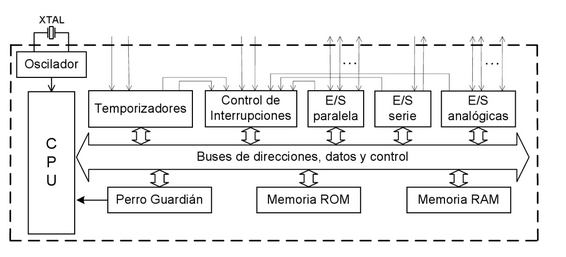
\includegraphics[scale = 1.0]{Material de Consulta/BloqMicro.PNG}
				\caption[Esquema de bloques de un microprocesador]{Esquema de bloques de un microprocesador}
				\label{BloqMicro}
			\end{figure}

				\subsubsection{Oscilador}
				Para poder realizar las operaciones internas el microcontrolador depende de un oscilador que genera los impulsos que permiten la sincronización de todas ellas. En la mayoría de los microcontroladores se utiliza como oscilador a un cristal de cuarzo debido a la gran estabilidad de frecuencia que ofrecen estos cristales ya que de estos dependen la velocidad de ejecucion de las tareas.

				\subsubsection{Watchdog Timer (Perro Guardián)}
				Es un recurso disponible en la mayoría de los microcontroladores, consta de un oscilador (puede ser el principal) y de un contador binario de N-bits. La salida del contador va conectada al circuito \textit{reset} del microcontrolador(\ref{BloqWDT}). El funcionamiento se define como un contador de pulsos que al llegar al desbordamiento reinicia el dispositivo, el fin de este bloque es que el programador evite el desbordamiento y por ende el reinicio del dispositivo, por ello se debe reiniciar el contador desde el programador. En cambio si existe un error en alguna parte del código que evita que se reinicie el contador del perro guardián este reiniciará el microcontrolador y será posible retomar el control y redirigir el programa por la ruta correcta.

				\begin{figure}[!htpb]
					\centering
					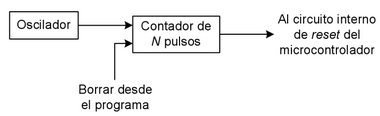
\includegraphics[scale = 1.0]{Material de Consulta/BloqWDT.PNG}
					\caption[Bloque WatchDog Timer]{Bloque WatchDog Timer}
					\label{BloqWDT}
				\end{figure}

				Es importante que cuando no se limpie el contador WDT a tiempo, se realice la acción de \textit{reset} ya que entonces significa que se ha encontrado un fallo en la secuencia de las instrucciones y para remediarlo se redirecciona a una direccion de memoria determinada y no una aleatoria como podría suceder en estos casos.

				En algunos microcontroladores como los PIC se señaliza la causa del reset por medio de bits de un registro del microcontrolador con lo cual se puede remediar el origen del fallo.

				\subsubsection{Reset}
				El reset es una función con la cual se inician los microprocesadores y los microcontroladores. Esta acción se ejecuta cuando una señal de reset es aplicada de manera manual a una terminal en el CI con lo cual se pone el contador de programa (PC) a un valor predeterminado comunmente 0 haciendo que el microprocesador comienze a ejecutar las instrucciones a partir de esa posición.

				En un microcomputador la señal de \textit{reset} se genera e forma manual al pulsar un botón o al iniciar el sistema (\textit{Reset} por encendido), sin embargo tambien pueden haber otras fuentes de \textit{reset} como lo son por "Fallo de Alimentación" o por "Desbordamiento del WatchDog Timer".

				El segundo caso, como se explicó anteriormente sucede cuando el contador WDT se desborda al no reiniciar el contador por lo que el microcontrolador ha perdido la secuencia de las instrucciones o ha entrado en un bucle demasiado largo. El primer caso sucede cuando el valor de voltaje cae por debajo del umbral de operación momentáneamente con lo que el capacitor se descarga parcialmente y se produce el reinicio del dispositivo.

				\subsubsection{Estado de Bajo Consumo}
				Una parte importante en los microcontroladores es la caracteristica de tener un bajo consumo de corriente ya que hay un gran número de aplicaciones que rquieren el uso de baterias como medio de alimentación por lo que un bajo consumo de corriente ayuda a una prolongada duración de la bateria.

				El consumo de corriente en el circuito se sustenta en el uso de compuertas CMOS que al mantenerse en un nivel lógico estático el consumo es prácticamente 0 y solo aumenta cuando el oscilador aumenta la frecuencia de las conmutaciones de los estados de las compuertas lógicas.

				Los microcontroladores comunmente se encuentran en este estado y únicamente se activan al ocurrir un evento externo, realizan una tarea y regresan a este estado por lo que se recomienda tener el microcontrolador con bajo consumo de corriente hasta que ocurra un evento que lo saque de ese letargo.

				\subsubsection{Memoria}
				La memoria en un microcontrolador es el lugar donde se almacenan el programa que se va a ejecutar y los datos y/o variables que va a utilizar. La memoria de datos es de lectura y escritura y los datos no permanecen en ella una vez que se suspende la alimentación al microcontrolador, es decir, la memoria es volátil (Memorias RAM estáticas). Algunos microcontroladores usan una memoria adicional externa de lectura y escritura no volátil como parte de la memoria de datos, para permitir almacenamiento de datos fijos, para este tipo de memorias se utilizan comunmente EEPROM.

				\begin{itemize}
					\item \textbf{RAM:} Esta es un tipo de memoria de lectura y escritura de alta velocidad. En la memoria RAM la información almacenada permanece estable indefinidamente mientras no se suprima la alimentación del microcontrolador.

					\item \textbf{ROM:} Si se usa memoria ROM ésta se graba durante la fabricación del dispositivo y no se puede alterar una vez almacenada, por ello el programa debe ser depurado. Los microcontroladores que utilizan este tipo de memorias son aquellos que se fabrican en grandes cantidades ya que su fabricación es bastante rentable gracias a su bajo costo. 

					\item \textbf{EEPROM:} Las memorias EEPROM son memorias no volátiles de lectura y escritura, donde la escritura se realiza por medios eléctricos y se puede lograr individualmente sin la necesidad de un borrado previo, sin embargo a pesar de ser reprogramables cuentan con un número finito de veces.

					\item \textbf{FLASH:} En las memorias FLASH se pueden realizar las operaciones de lectura y escritura celda por celda, pero a diferencia de las anateriores se requiere primero borrar la información de la celda antes de escribir en ella y estas deben borarse por bloques de celdas colocando a 0. A menudo las operaciones de ecritura de información se debe realizar un proceso de lectura-borrado-escritura del bloque de celdas donde se desea escribir la información. Todas las operaciones de borrado, lectura y escritura se realizan con la misma tensión de voltaje
				\end{itemize}

			\subsection{Arquitecturas CISC y RISC}
			CISC (Complex Instruction Set Computer) y RISC (Reduced Instruction Set Computer) son dos modelos de computadoras visto desde el repertorio de instrucciones que repercuten en el modelo de arquitectura de la CPU y como lo dice su nombre las computadoras CISC tiene una mayor cantidad de instrucciones miestras que el RISC posee una menor cantidad.

			Las arquitecturas CISC predominaba en un inicio debido a la ambición de hacer los microprocesadores y microcontroladores los más potente posibles. Debido a la complejidad que fue aumentando lo hizo también la complejidad de la CPU y por ende se le debió dedicar un mayor espacio en el circuito integrado a la decodificadción y ejecución de las instrucciones.

			Por el contrario las RISC tienen un repertorio corto de instrucciones sencillas que pueden realizar operaciones simples pero a alta velocidad. La complejidad del CPU disminuye, así que a frecuencia del oscilador puede aumentar y así mejorar la velocidad de ejecución de las operaciones. Esto támbien apoya en su fabricación siendo más sencillos y baratos de producir, por ello esta arquitectura ha sido la predominante en microcontroladores PIC.

		\section{PIC32MZ2048EFM100}
		Es un microcontrolador de 32-bits que permite la conectividad embebida con una unidad de Punto Flotante\cite{PIC32MZ}, esta familia de microcontroladores poseen una gran cantidad de puertos de comunicación lo que permite que sea una opción bastante adecuada para proyectos en los que se necesite el intercambio de información entre varios dispositivos.

		La especificaciones del microcontrolador se pueden ver en la tabla.

		\begin{table}[!htpb]
				\centering
				\begin{tabular}{ l | c }
					\textbf{Nombre} & \textbf{Valor} \\
					\hline
					Familia & PIC32MZEF \\
					\hline
					Velocidad Max CPU [MHz] & 200 \\
					\hline
					Tamaño de Memoria Programable [KB] & 2048 \\
					\hline
					SRAM [KB] & 512\\
					\hline
					Auxiliary Flash [KB] & 160 \\
					\hline
					Crypto Engine & Yes \\
					\hline
					Range Temperatura [°C] & -40 to 125 \\
					\hline
					Rango de Voltaje Operacional [V] & 2.2 to 3.6 \\
					\hline
					Direct Memory Access Channels & 8 \\
					\hline
					Canales SPI & 6 \\
					\hline
					Canales I2C & 5 \\
					\hline
					Interfaz CODEC (I2S,AC97) & Yes \\
					\hline
					Peripheral Pin Select / Pin Muxing & Yes \\
					\hline
					Ethernet & 10/100 Base-TX Mac \\
					\hline
					Número de Puertos Ethernet  & 1 \\
					\hline
					Número de Modulos USB & 1 \\
					\hline
					Interfaz USB & High Speed \\
					\hline
					Números de Modulos CAN & 2 \\
					\hline
					Tipo de Modulos CAN & CAN \\
					\hline
					Entrada ADC & 40 \\
					\hline
					Resolucion Max ADC (Bits) & 12 \\
					\hline
					Max Rango de Muestreo ADC [ksps] & 18000 \\
					\hline
					Entradas de Captura & 9 \\
					\hline
					Standalone Output Compare/Standard PWM & 9 \\
					\hline
					Max 16-bit Digital Timers & 9 \\
					\hline
					Parallel Port & PMP \\
					\hline
					Number of Comparators & 2 \\
					\hline
					Internal Oscillator & 8 [MHz], 32 [kHz] \\
					\hline
					Hardware RTCC/RTC & Yes \\
					\hline
					Max I/O Pins & 78 \\
					\hline
					Pincount & 100 \\
					\hline
					Serial Quad Interface & Yes \\
				\end{tabular}
				\caption{Especificaciones PIC32MZ2048EFM100}
		\end{table}

		En particular esta familia de microcontroladores posee perifericos que operan a una mayor frecuencia que los microcontroladores tipicos usados para los sistemas embebidos. Esto es posible gracias al microprocesador que posee la CPU el cual contiene varios bloques lógicos que trabajan en conjunto en paralelo, proviendo un alto rendimiento de procesamiento.

		\section{Medidor de Energía ADE7880}
		Este Circuito Integrado es un medidor de energía eléctrica trifasica de alta precisión, con interfaces de comunicación serial I$^2$C y SPI. Es adecuado para la medición de energía electrica activa, reactiva y aparente en varias configuraciones trifásicas, además posee registros de muestreo de formas de onda para todas las salidas del Convertidor Análogico Digital incluido en el CI\footnote{Circuito Integrado ADE7880 renombrado asi a partir de aqui para simplificar.}.

			\subsection{Gestion de Energía}
			Este CI posee 4 modos de energía determinados por el estado de los pines PM0 y PM1 estros proveen total control sobre el chip y gracias a que poseen resistencias pull-up internas se pueden copnectar facilmente al microcontrolador.

			Los modos de operación son:

			\begin{table}[!htpb]
				\centering
				\begin{tabular}{ l | c | c}
					\textbf{Modo de Energía} & \textbf{PM1} & \textbf{PM0}\\
					\hline
					PSM0 & 0 & 1 \\
					PSM1 & 0 & 0 \\
					PSM2 & 1 & 0 \\
					PSM3 & 1 & 1 \\
				\end{tabular}
				\caption[Modos de Suministro de Energía]{Configuración de los pines PM para los modos de suministro de energía}
			\end{table}

			\begin{itemize}
				\item \textbf{PSM0 (Normal Power Mode):} Este es el modo de operación completamente funcional.
				Si el medidor de energía se encuentra en cualquiera de los otros modos y se cambia a este todos los regitros automáticamente son reiniciados a sus valores iniciales, con excepción del registro LPOILVL\footnote{Registro del límite de sobrecorriente durante el modo PSM2.} y el registro CONFIG2\footnote{Registro de configuración de armónicos.}.

				Cuando se realiza la transición de un modo de energía a otro el CI cambia el estado del pin $\overline{IRQ1}$ a bajo y el bit 15 (RSTDONE) en el registro STATUS1 a alto, especialmente este último es el que indica el fin de la transición ya que durante es 0.

				\item \textbf{PSM1 (Reduced Power Mode):} En este modo el CI mide los valores absolutos promedio de las 3 fases de corriente para almacenarlos en los registros \textit{xIMAV} \footnote{\textit{x:} Canal de corriente  A. B, C.}. 
				Este modo es útil al usar una batería externa. Los puertos de comunicación serial estan activos y se puede utilizar para leer los registros \textit{xIMAV}, sin embargo, a pesar de poder leer estos registros para los demás registros del CI no se garantizan que los valores sean correctos.

				Al entrar en este modo despues de haber estado en en el PSM0 entonces el cálculo de valor absoluto promedio inicia sin retrasos. Los registros \textit{xIMAV} son accesibles en cualquier momento después de que el pin $\overline{IRQ1}$ ha cambiado a un valor de 0 (indicando el inicio del cómputo de valores absolutos promedio).

				\item \textbf{PSM2 (Low Power Mode):} Los puertos de comunicación no son funcionales en eeste modo, se reduce el consumo requerido para monitorear la corriente cuando no hay entrada de voltaje y la fuente de voltaje es provista por una bateria externa.

				Si el pin $\overline{IRQ0}$ está en un nivel lógico bajo al acabar el periodo de medición, entonces significa que todas las fases de corriente se meantuvieron por debajo del límite y, por lo tanto, no hay corriente fluyendo por el sistema, en este punto el microcontrolador externo pone el CI en modo de de espera. Si en cambio el pin $\overline{IRQ1}$ es el que se encuentra en bajo, entonces significa que por lo menos una entrada de corriente está por encima del límite definido y hay corriente fluyendo por el sistema a pesar de que no hay voltaje presente en los pines del CI. Esta situación se conoce como falta neutra, en este punto el microcontrolador externo coloca el CI en el modo PSM1. No es recomendable usar este modo si los registros de ganancia\footnote{PGA1[2:0].} son diferentes a 1 ó 2.

				\item \textbf{PSM3 (Sleep Mode):} En este modo la mayoría de los circuitos internos se encuentran apagados y el consumo de corriente se mantiene a su más bajo nivel. Los puertos I$^2$C, SPI Y HSDC no son funcionales, además los pines de $\overline{RESET}$, MOSI/SDA, SCLK/SCI y $\overline{SS}$/HSA deben permanecer en alto.
			\end{itemize}

			\subsection{Procedimiento de Encendido}
			El ADE7880 posee un chip interno que monitorea la fuente de alimentación (VDD). En el encendido el dispositvo permanece inactivo hasta que VDD alcanza los 2.0[V]$\pm$10\%. Al sobrepasar este límite el monitor mantiene el dispositivo en inactivo por 26[ms] para permitir alcanzar el voltaje de 3.3[V]$\pm$10\% a la fuente de voltaje.

			\begin{figure}[!htpb]
				\centering
				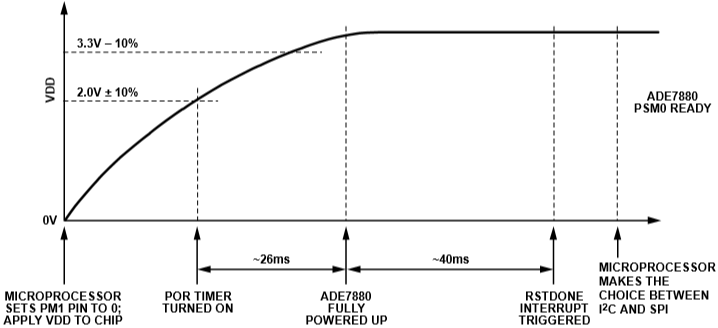
\includegraphics[scale = 0.8]{Material de Consulta/Encendido.PNG}
				\caption[Encendido del ADE7880]{Procedimiento de encendido}
				\label{ADEOn}
			\end{figure}

			Los pines PM0 y PM1 tienen resistencias pull-up, pero es necesario el colocar PM1 en un nivel lógico bajo ya sea por hardware (colocando a tierra) ó a travez del microcontrolador antes de encender el chip, para asegurar que el dispositivo se inicie en PSM0. El tiempo de encendido es de al rededor de 40[ms] tiempo en el cual el pin de $\overline{RESET}$ debe permanecer en un nivel lógico alto.

			Al iniciar en en modo PSM0 el puerto activo es el I$^2$C, si se desea cambiar el puerto de comunicación se tiene que alternar el pin $\overline{SS}$/HSA 3 veces de un nivel lógico de voltaje alto a un nivel de voltaje bajo. Cuando se decide usar un puerto de comunicación este debe bloquearse para evitar que durante la comunicación ó combio de modo de energía se alterne por el otro puerto y se pierda la comunicación. Para ello si el puerto activo es el I$^2$C se debe escribir un 1 el bit 1 (I2C\_LOCK) del registro CONFIG2 en caso contrario si el puerto activo es el SPI entonces cualquier escritura al registro CONFIG2 bloqueará este puerto como el activo. En ambos casos el cambio por el otro puerto de comunicación no es posible hasta que se haga un reinicio de hardware o se apague y vuelva a encender el sistema.

			Inicialmente el CI se encuentra en modo de reposo y, por lo tanto, no ejecuta ninguna instrucción, es en este punto donde todos los registros necesarios para la ejecución del programa deben iniciarse. Si el voltaje cae por debajo de los 2.0[V]$\pm10\%$ este entra en estado inactivo y ninguina medición ó cómputo es ejecutada.

			\subsection{Hardware Reset}
			Este tipo de reset se logra al tener el CI en el modo PSM0 y colocando el pin de $\overline{RESET}$ en un nivel de voltaje bajo, en otros modos de energía el pin no tiene función. Si entonces el pin es alternado de alto-bajo-alto con 10[ms] de retraso entre cambio. Durante el proceso de reinicio el pin $\overline{IRQ1}$ permanece en 1, al termino del proceso este pin es colocado a 0 y todos los registros son devueltos a sus valores iniciales de fábrica. 

			El reinicio por Hardware devuelve el puerto I$^2$C como canal principal de comunicación.

			\subsection{Software Resest}
			Al igual que el reset por Hardware estaopción solo esta disponible durante el modo PSM0. Para iniciar el reset por Software se utiliza el bit 7 en el registro CONFIG, inicialmente este bit se encuentra en 0, y si es cambiado a 1 entonces entra en modo de Reset, el cual regresa a valores iniciales a la mayoria de los registros, la seleccion de puerto de comunicación se mantiene si se ha bloqueado de manera correcta. Los únicos valores que mantienen sus valores son CONFIG2 y LPOILVL.

			\subsection{Operación del ADE7880}
				\subsubsection{Entradas analógicas}
				Se tienen 7 entradas analógicas que forman los canales de corriente y voltaje. Los canales de corriente constan de 4 pares de entradas IxP/IxN\footnote{x: Canales A, B, C y N respectivamente} diferenciales los cuales tienen un máximo de señal $\pm$0.5[V] e igual con respecto a la señal en AGND\footnote{Referencia a tierra para el circuito analógico.}.

				\begin{figure}[!htpb]
					\centering
					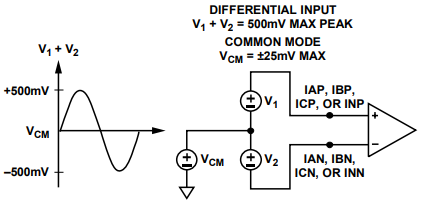
\includegraphics[scale = 1.0]{Material de Consulta/EntAnCrrnt.PNG}
					\caption[Entradas analógicas de corriente]{Esquema de entradas analógicas de corriente}
					\label{EntCrnt}
				\end{figure}

				Todas las entradas poseen un Amplificador Programable de Ganancia (PGA por sus siglas en inglés) con una selección de 1, 2, 4, 8 ó 16. Las ganancias presentes en IA, IB e IC se colocan en un registro diferente a IN\footnote{Entrada analógica del canal de corriente neutral.} para obtener una ganancia diferente a las 3 primeras.

				\begin{figure}[!htpb]
					\centering
					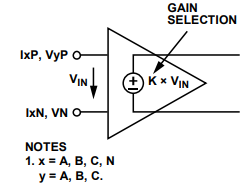
\includegraphics[scale = 1.0]{Material de Consulta/AmpGan.PNG}
					\caption[Amplificadores de Ganancia]{Esquema de los amplificadores de ganancia en las entradasa analógicas}
					\label{AmpGan}
				\end{figure}

				El canal de voltaje tiene 3 entradas de voltaje de un sólo extremo, con una entrada máxima de  $\pm$0.5[V] con respecto a VN\footnote{Entrada analógica del canal de voltaje neutral.},
				de igual manera estas entradas tienen una entrada de señal máxima de $\pm$0.5[V] con respecto a AGND.

				\begin{figure}[!htpb]
					\centering
					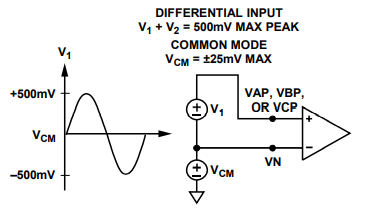
\includegraphics[scale = 1.0]{Material de Consulta/EntAnVlt.PNG}
					\caption[Entradas analógicas de Voltaje]{Esquema de entradas analógicas de voltaje}
					\label{EntVolt}
				\end{figure}

				\subsubsection{Convertidor Analógico Digital}
				A las entradas de los canales de corriente y voltaje se tienen Convertidores Analógicos Digitales $\Sigma$-$\Delta$, estos se encuentran activos en el modo PSM0, y en el PSM1 solo los que miden los canales de corriente se encuentran activos a excepcion del canal de corriente neutral. En los otros modos no estan activos ninguno de los ADC\footnote{Convertidor Analógico Digital.}.

				\begin{figure}[!htpb]
					\centering
					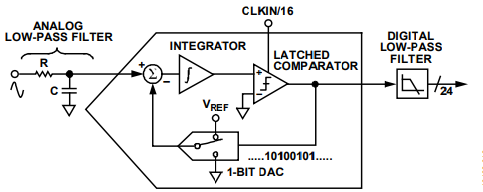
\includegraphics[scale = 1.0]{Material de Consulta/ADC_SigDel.PNG}
					\caption[Convertidor Analógico Digital]{Convertidor Analógico Digital}
					\label{ADCSigDel}
				\end{figure}

				El módulo $\Sigma$-$\Delta$ convierte la señal de entrada en un flujo en serie de "1" y "0" a un tiempo determinado por el reloj de muestreo (En el ADE7880 este reloj es de 1.024[MHz]). El DAC\footnote{Convertidor Digital Analógico.} de 1-bit en el bucle de retroalimentación es llevado por el flujo de datos en serie, entonces la la salida del DAC es sutraida de la señal de entrada. Si el bucle de ganancia es lo suficientemente alto el valor promedio de la salida del DAC puede aproximarse al nivel de la señal de entrada. El promedio es pasado entonces a un filtro digital pasa-bajas que produce una palabra de 24-bits proporcional al nivel de la señal de entrada.

				\subsubsection{Filtro Antialias}
				Este filtro se encuentra a la entrada del ADC y su función es la de prevenir el solapamiento que se presenta en todos los sistemas de muestreo.

				Para sensores de corriente convencionales es recomendable usar filtros RC\footnote{RC: Resistor Capacitor.} con una frecuencia de corte de 5[kHz] para que la atenuación sea suficiente para eliminar los efectos de solapamiento para sensores de corriente convencionales.

				\subsubsection{Función de Transferencia de los ADC}
				Todos los ADC en el CI estan diseñados para producir el mismo nivel de señal de la salida en el código de 24-bits con signo a la salida. El código del ADC puede variar entre 0x800000 (-8,388,608) y 0x7FFFFF (8,388,607), esto es equivalente a una señal de entrada de $\pm$0.787[V], por lo tanto no debe excederse el rango nominal especificado de $\pm$0.5[V]. Las señales se muestrean a una velocidad de 8[kSPs]\footnote{kSPs: Mil muestras por segundo (Kilo Samples per second).}.

%-----------------------------------------------------------------------------%
			\subsection{Interfaces de Comunicación}
			El ADE7880 posee 3 puertos de comunicación serial SPI, I$^2$C Y HSDC, sin embargo por la configuración de los pines solo se pueden usar 2 tipos de configuraciones, una utilizando el puerto SPI únicamente y la segunda es usando los puertos I$^2$C Y HSDC.

			Se incluyen un conjunto de 3 registros que permiten verificar la comunicación con el CI. Los regsitros LAST\_OP (Address 0xEA01), LAST\_ADD (Address 0xE9FE) and LAST\_RWDATA se encargan de almacenar los datos, la dirección de registro y la naturaleza del acceso al registro (Lectura/Escritura) de la última comunicación exitosa respectivamente. El registro LAST\_RWDATA tiene 3 diferentes direcciones dependiendo de la longitud del registro de la última comunicación.

			\begin{table}[!htpb]
				\centering
				\begin{tabular}{ l | c }
					\textbf{Tipo de comunicación} & \textbf{Dirección de registro} \\
					\hline
					Lectura/ Escritura de 8-Bit & 0xE7FD \\
					Lectura/ Escritura de 16-Bit & 0xE9FF \\
					Lectura/ Escritura de 32-Bit & 0xE5FF \\
				\end{tabular}
				\caption[Registros de última escritura]{Direcciones de los registros de última escritura (LAST\_RWDATA)}
			\end{table}

			Después de cada comunicación exitosa los registros se actualizan con la información de la operación, 0xCA si fue escritura y 0x35 si es escritura y el dato que se leyó o escribió. Las operciones no completadas no se reflejan en estos registros asi como cuando se leen estos registros.

			\subsubsection{SPI (Serial Peripheral Interface)}
			El SPI de este CI siempre es esclavo en la comunicación y consiste en 4 pines de comunicación SCLK, MOSI, MISO Y SSA.

			El reloj para la transferencia de datos debe aplicarse al pin SCLK y todas las transferencias de datos se sincronizan con este reloj. El intercambio de información entrante en el CI se realiza en el pin MOSI en los flancos descendentes del reloj serial y el CI lo muestrea en los flancos ascendentes del reloj. Por el contrario la información saliente del CI se transfiere por el pin MISO en los flancos descendentes del reloj serial y el dispositivo maestro muestrea la información en los flancos ascendentes. El bit más significante de la palabra es intercambiado a la entrada. La másima frecuencia del reloj serial soportada por esta interfaz es de 2.5[MHz], el pin MISO se mantiene en alta impedancia mientras no hay intercambio de información.

			EL pin $\overline{SS}$ es utilizado para seleccionar entra más de un dispositivo si es que los hay. Para poder utilizar el dispositivo y realizar la comunicación entre ete y el dispositivo maestro este pin debe llevarse a un voltaje lógico bajo y permanecer así mientras dure la comunicación. Al cambiar el nivel lógico de este pin aborta la transferencia y para iniciar una nueva este se debe volver a poner a un voltaje lógico bajo.

			\subsubsection{I$^2$C (Inter Integrated Circuits)}
			Este CI posee una interfaz I$^2$C para la comunicación, implementada completamente como un hadware esclavo. El pin de intercambio de información SDA se encuentra localizado en el pin 38 y se encuentra compartido con el pin MOSI del puerto SPI, de igual manera el reloj serial SCL se encuentra compartido con el reloj serial del puerto SPI en el pin 36. La máxima frecuencia soportada por el reloj serial es de 400[kHz].

			La secuencia de transferencia del sistema I$^2$C consiste en el dispositivo maestro generando un condición de inicio para la transferencia cuando el bus se encuantra desocupado. El dispositivo maestro entonces transmite la direccion del dispositivo esclavo (0x70) y la dirección del regitro de la transferencia de datos en la transferencia de dirección inicial si el dispositivo esclavo reconoce entonces empieza la transferencia de datos. Esto continua hasta que el maestro emite una condición de parada y el bus queda de nuevo desocupado.

			\subsubsection{HSDC (High Speed Data Capture)}
			Debido a que para este proyecto es necesario el recopilar una gran cantidad de muestras a alta velocidad la documentación del Circuito Integrado ADE7880 recomienda, para la lectura de estos registros en específico, utilizar una interfaz propia de Analog Devices para este circuito llamada High Speed Data Capture (Captura de Datos a Alta Velocidad) por lo que es necesario configurar el microprocesador de manera que se pueda usar la comunicación I$^2$C como interfaz serial principal y la comunicación HSDC como secundaria usando el canal SPI del microcontrolador como esclavo, que recibirá toda la información de los registros de voltaje y corriente enviados por esta interfaz.

		\section{Entorno de Desarrollo MPLABX}
		Microchip provee un entorno de desarrollo y un compilador 
			\subsection{Herramienta de configuración MPLAB Harmony}

%%%%%%%%%%%%%%%%%%%%%%%%%%%%%%%%%%%%%%%%%%%%%%%%%%%%%%%%%%%%%%%%%%%%%%%%%%%%%%%
%%%%%%%%%%%%%%%%%%%%%%%%%%%%%%%%%%% FIRMWARE %%%%%%%%%%%%%%%%%%%%%%%%%%%%%%%%%%
%%%%%%%%%%%%%%%%%%%%%%%%%%%%%%%%%%%%%%%%%%%%%%%%%%%%%%%%%%%%%%%%%%%%%%%%%%%%%%%
		\section{Firmware}
			\subsection{Inicialización}
			La programación del proyecto se realiza por parte del entorno de desarrollo de Microchip MPLAB X, mientras que la conficuración de los puertos se realiza con la herramienta proporcionada por el mismo MPLAB Harmony debido a que la configuración manual sería demasiado complicada debido a la cantidad de puertos, pines y servicios disponibles por parte del microcontrolador. ya que esta es una actualización del módulo de medición de energía por lo que la inicialización esta parcialmente completa, sin embargo al realizar el cambio de canal de comunicación principal de SPI (\ref{ConfigSPI}) a I2C(\ref{ConfigI2C}) y HSDC(Este puerto utiliza la interfaz SPI del microcontrolador por lo que se reconectan los pines pero se deja la configuración ) se cambió las configuraciones de estos canales. Todas las demás siguieron igual a como se tenían en la primer versión del módulo.

			\begin{figure}[!htpb]
				\centering
				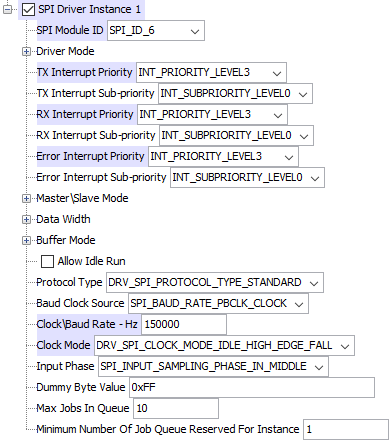
\includegraphics[scale = 0.8]{Pruebas de Comunicación/ConfigSPI.PNG}
				\caption[Configuración SPI del PIC32MZ]{Configuración SPI del PIC32MZ}
				\label{ConfigSPI} 
				\hfill \break
				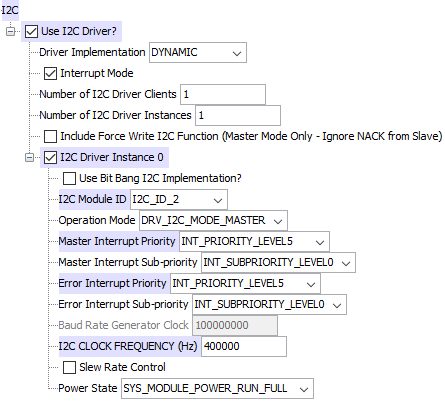
\includegraphics[scale = 0.8]{Pruebas de Comunicación/ConfigI2C.PNG}
				\caption[Configuración I2C del PIC32MZ]{Configuración I2C del PIC32MZ}
				\label{ConfigI2C}
			\end{figure}

			\subsection{Configuración del puerto I$^2$C}
			Este puerto se activa al encender el dispositivo o al realizar un reinicio de hardware, entonces el puerto I$^2$C queda seleccionado como interfaz de comunicación. Para evitar que al hacer cambios en el nivel de voltaje del pin $\overline{SS}$/HSA se cambie a la interfaz de comunicación SPI, se debe bloquear el puerto I$^2$C para ello se debe poner a 1 el Bit 1 (I2C\_LOCK) del registro CONFIG2, esto previene que al realizar cambios de voltaje en el pin $\overline{SS}$/HSA y el cambio a SPI no es posible hasta que se realize un reinicio de hardware o se reinicie todo el sistema.

			\begin{table}[ht]
				\centering
				\begin{tabular}{c | c | c}
					\textbf{Bit} & \textbf{Mnemonico} & \textbf{Valor predeterminado} \\
					\hline
					0 & EXTREFEN & 0 \\
					\hline
					1 & I2C\_LOCK & 1 \\
					\hline
					7:2 & Reservados & 0 \\
				\end{tabular}
				\caption[Valores de bloqueo del puerto I$^2$C]{Valores del registro CONFIG2 que se deben transmitir para bloquear el puerto I$^2$C}
			\end{table}

			Este registro se accesa como si fuera un registro de 8-Bits por lo que los 6 Bits más significativos deben permanecer como 0. En este caso en particular se transmite 0x02 a la dirección de registro 0xEC01.

			\subsection{Configuración del puerto HSDC}
			Para configurar el puerto HSDC se debe escribir primero al registro HSDC\_CFG [0xE706] a traves del puerto I$^2$C la configuración con la que se van a estar enviando los datos a traves del puerto HSDC. Ya que se configura el puerto se habilita colocando el bit 6 (HSDCEN) en el registro CONFIG [0xE618] a 1, con esto se activa la comunicación.

			La configuracion que se ha decidido usar es tener el reloj a 8[MHz] con la transmision de registros en paquetes de 32-bits, no se agrega una brecha de 7 ciclos de reloj entre transmisiones y unicamente se transmitira el contenido de los registros de voltaje y corriente: IAWV, VAWV, IBWV, VBWV, ICWV, VCWV, e INWV, lo que permite que se realice la comunicación de manera más rápida. El pin de selccion de esclavo ($\overline{SS}$ ó Chip Select) se mantiene como activo en bajo. %AUN SE ESTA PROBNADO SI FUNCIONARIA CON ACYIVO E BAJO O SE DEBE USAR COMO ACTIVO EN ALTO
%%%%%%%%%%%%%%%%%%%%%%%%%%%%%%%%%%%%%%%%%%%%%%%%%%%%%%%%%%%%%%%%%%%%%%%%%%%%%%%
%%%%%%%%%%%%%%%%%%%%%%%%%%%%%%%%%% RESULTADOS %%%%%%%%%%%%%%%%%%%%%%%%%%%%%%%%%
%%%%%%%%%%%%%%%%%%%%%%%%%%%%%%%%%%%%%%%%%%%%%%%%%%%%%%%%%%%%%%%%%%%%%%%%%%%%%%%
	\chapter{Resultados}
	Como se explicó al principio el desarrollo de este proyecto se pensó como una mejora a los medidores de energía anteriormente fabricados por el Instituto de Ingeniería por lo que este, solo se centró únicamente en la lectura de muestras a alta velocidad por parte del microcontrolador.

		\section{Lectura de Datos Usando el Canal SPI}
		En un principio el sistema medidor de energía estaba pensado para realizar la comunicación entre el microprocesador y el medidor ADE7880 con interfaz SPI sin embargo al momento de realizar las primeras pruebas, los registros correspondientes a los canales de medición de voltaje y corriente, pasado un tiempo los valores que se recuperan de los registros pierden coherencia lo que hace que los resultados sean inutiles para su análisis.

		La lectura de los registros se configuró para que el microprocesador lo realizara a la mayor velocidad posible utilizando un reloj de 150000[Hz] por el canal 6 SPI \ref{ConfigSPI}.

		En la siguiente gráfica \ref{ComSPI} se puede ver como la velocidad de comunicación es bastante rápida al leer los valores de registro a pesar de tener que leer el registro DREADY para asegurarse que los registros de voltaje y corriente esten listos se obtenían demasiado rápido, pero como se había mencinado estos valores no demostraban valores que puedan ser útiles.

		\begin{figure}[!htpb]
			\centering
			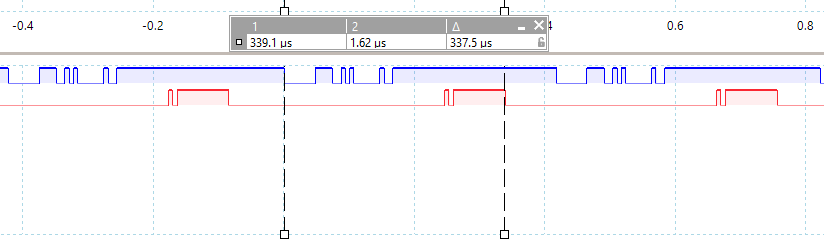
\includegraphics[scale = 0.5]{Pruebas de Comunicación/DREADY_TimeComp.PNG}
			\caption[Comunicación SPI con los registros de voltaje y corriente]{Comunicación SPI con los registros de voltaje y corriente}
			\label{ComSPI} 
		\end{figure}

		Como se pueden ver en las graficas de voltaje (Graficas \ref{CanalVoltaje}) y corriente (Graficas \ref{CanalCorriente}) al usar el canal SPI para muestrear los registros de voltaje y corriente de los 3 canales estos entregaban valores que no reflejaban la energía que se suministraba y en algunos casos ni siquiera se actualizaban los valores que el dispositivo tiene inicialmente, ya que las pruebas que se hacían se realizaban con un simulador de voltaje y corriente controlado con lo cual era posible conocer el valor que se deseaba obtener.

		Después de realizar un par de pruebas más y obtener valores similares en todas las pruebas y siguiendo la recomendación que el manual del dispositivo para la lectura de esos registros se decidió cambiar el canal de comunicación de SPI por el HSDC con el cual se planea tener una lectura más rápida de los registros así como poder mantener la comunicación únicamente con los registros de voltaje y corriente de manera continua sin interaciones con los otros módulos del sistema de medición de energía.

		\begin{figure}[!htbp]
			\subfigure[Canal de Voltaje A]{
				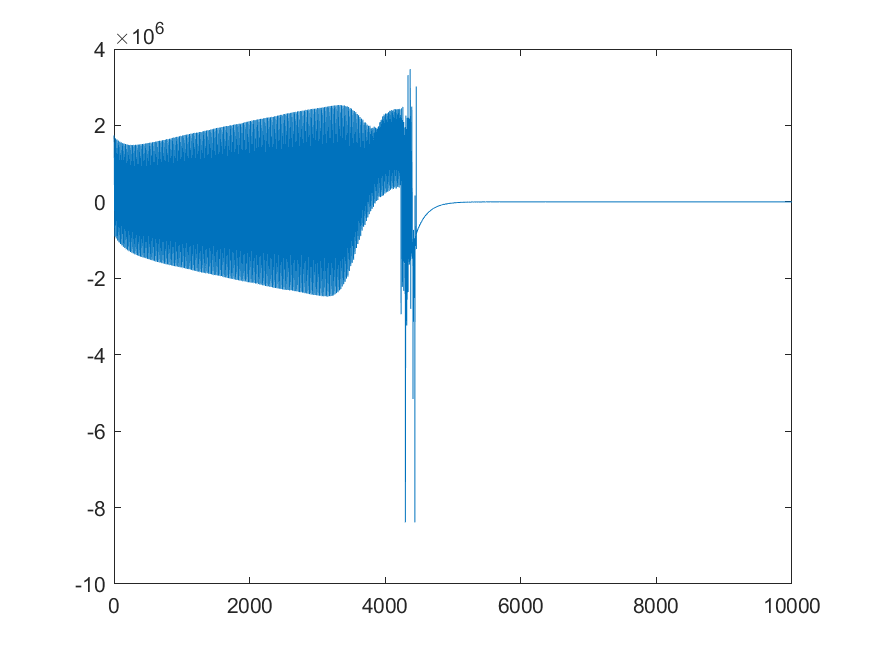
\includegraphics[scale = 0.6]{Pruebas de Muestreo/QS_140220.png}
			}
			\subfigure[Canal de Voltaje B]{
				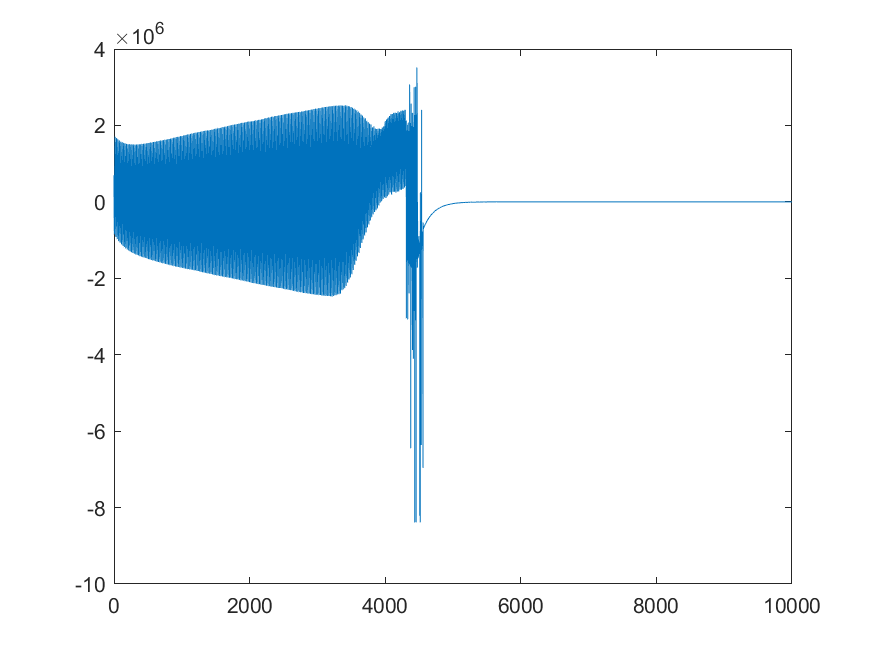
\includegraphics[scale = 0.6]{Pruebas de Muestreo/QS_140220-000000.png}
			}
			\subfigure[Canal de Voltaje C]{
				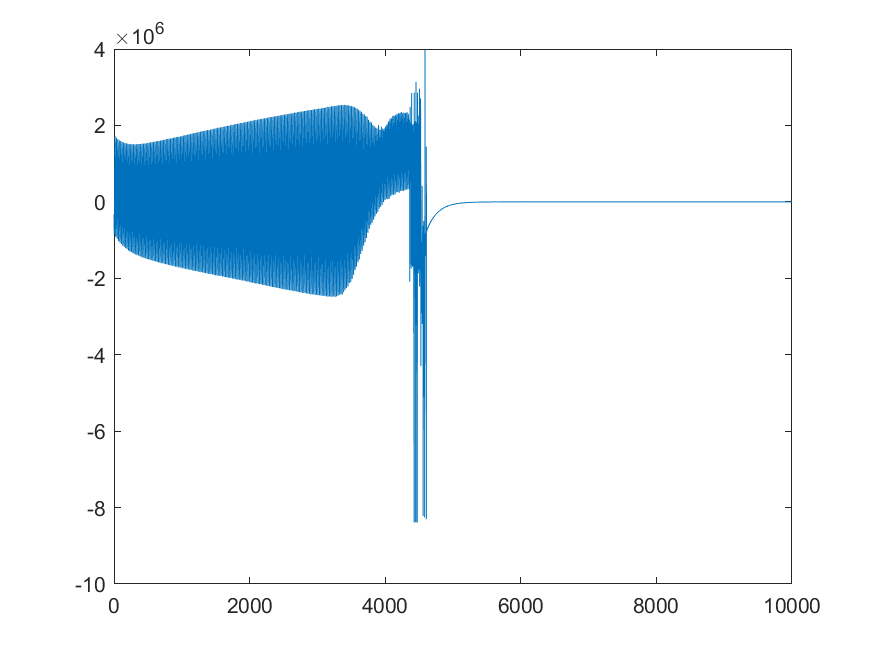
\includegraphics[scale = 0.6]{Pruebas de Muestreo/QS_140220-000001.png}
			}
			\caption[Gráficas de la primer prueba de los Canales de Voltaje]{Gráficas de la primer prueba de los Canales de Voltaje}
			\label{CanalVoltaje}
		\end{figure}

		\begin{figure}[!htbp]
			\subfigure[Canal de Corriente A]{
				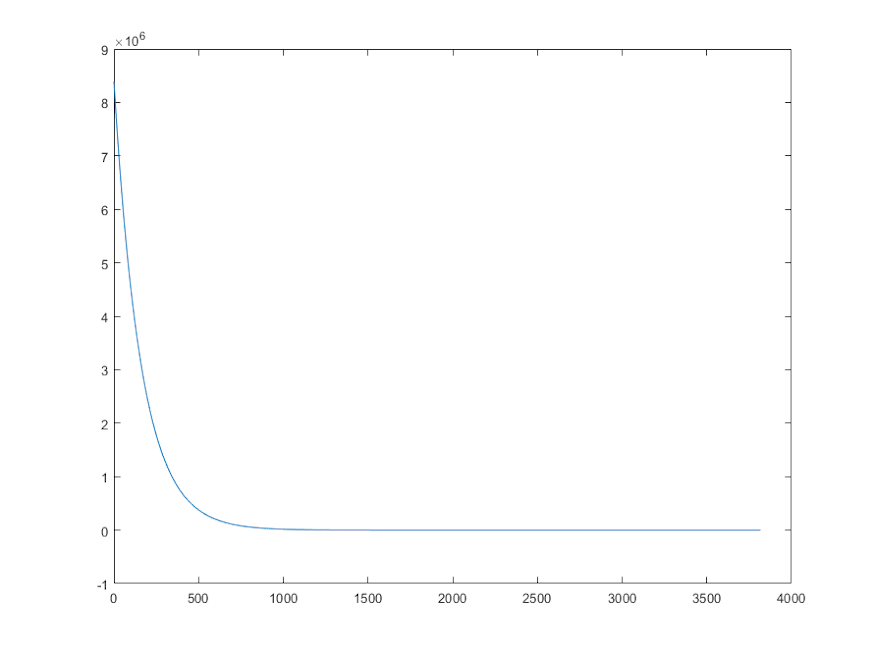
\includegraphics[width = 8.6cm, height = 6.7cm]{Pruebas de Muestreo/QS.png}
			}
			\subfigure[Canal de Corriente B]{
				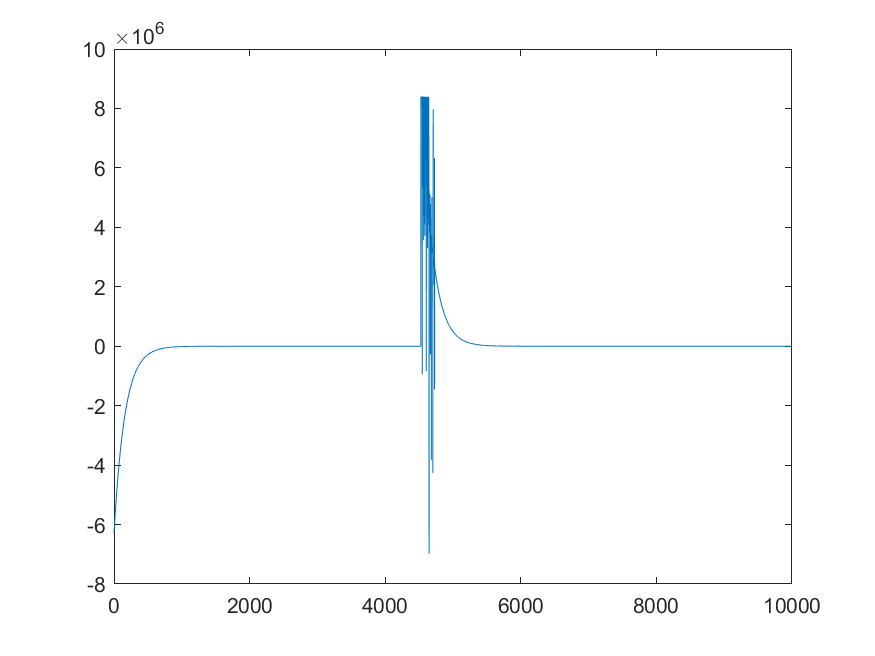
\includegraphics[scale = 0.6]{Pruebas de Muestreo/QS_140221.png}
			}
			\subfigure[Canal de Corriente C]{
				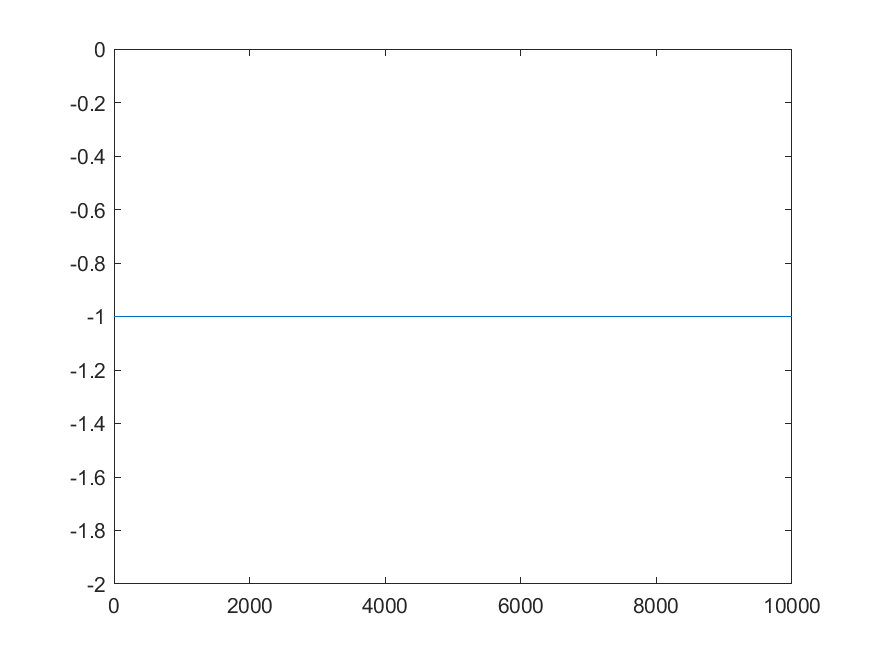
\includegraphics[scale = 0.6]{Pruebas de Muestreo/QS2.png}
			}
			\caption[Gráficas de la primer prueba de los Canales de Corriente]{Gráficas de la primer prueba de los Canales de Corriente}
			\label{CanalCorriente}
		\end{figure}

		\section{Lectura de Datos usando el canal HSDC}
		Las primeras pruebas que se realizaron usando este canal de comunicación inicia de manera correcta al configurar los valores necesarios en el registro correspondiente del ADE7880, se comprobó usando el osciloscopio que los paquetes de datos se envíen y reciban de manera correcta por el canal I2C para despues comprobar que el puerto HSDC realmente envíe información.
		%%%%%%%%%%%%%%%%%%%%%%%%%%%%%%%%%%%%%%%%%%%%%%%%%%%%%%%%%%%%%%%%%%
		%COLOCAR IMAGEN DEL OSCILOSCOPIO DE LOS DATOS ENVIADOS POR EL I2C%
		%%%%%%%%%%%%%%%%%%%%%%%%%%%%%%%%%%%%%%%%%%%%%%%%%%%%%%%%%%%%%%%%%%
		Al iniciar el DSP se comprobó que el puerto HSDC enviaba la información proveniente de los registros de corriente y voltaje del medidor de energía.
		%%%%%%%%%%%%%%%%%%%%%%%%%%%%%%%%%%%%%%%%%%%%%%%%%%%%%%%%%%%%%%%%%%
		%COLOCAR IMAGEN DEL OSCILOSCOPIO DE LOS DATOS ENVIADOS POR EL HSDC%
		%%%%%%%%%%%%%%%%%%%%%%%%%%%%%%%%%%%%%%%%%%%%%%%%%%%%%%%%%%%%%%%%%%
	
	\chapter{Conclusiones}

	\chapter{Glosario}
	Frecuencia de corte ($\omega$C) o también llamada frecuencia de esquina o frecuencia crítica. Es  la  frecuencia  donde  la  respuesta  en  amplitud  está  3  dB  por  abajo  del  valor  de  la banda de paso.
	
	\bibliography{Bibliografia}
	\bibliographystyle{apalike}
	
	\appendix
	\chapter{Hojas de Datos de la Familia PIC32MZ}
		\includepdf[pages = {1,5,6,19,327,365,366,652,653,654,657,658,659,660,676,677,678,679}]{Material de Consulta/PIC32MZ}

	\chapter{Hojas de Datos del Medidor de Energía ADE7880}
		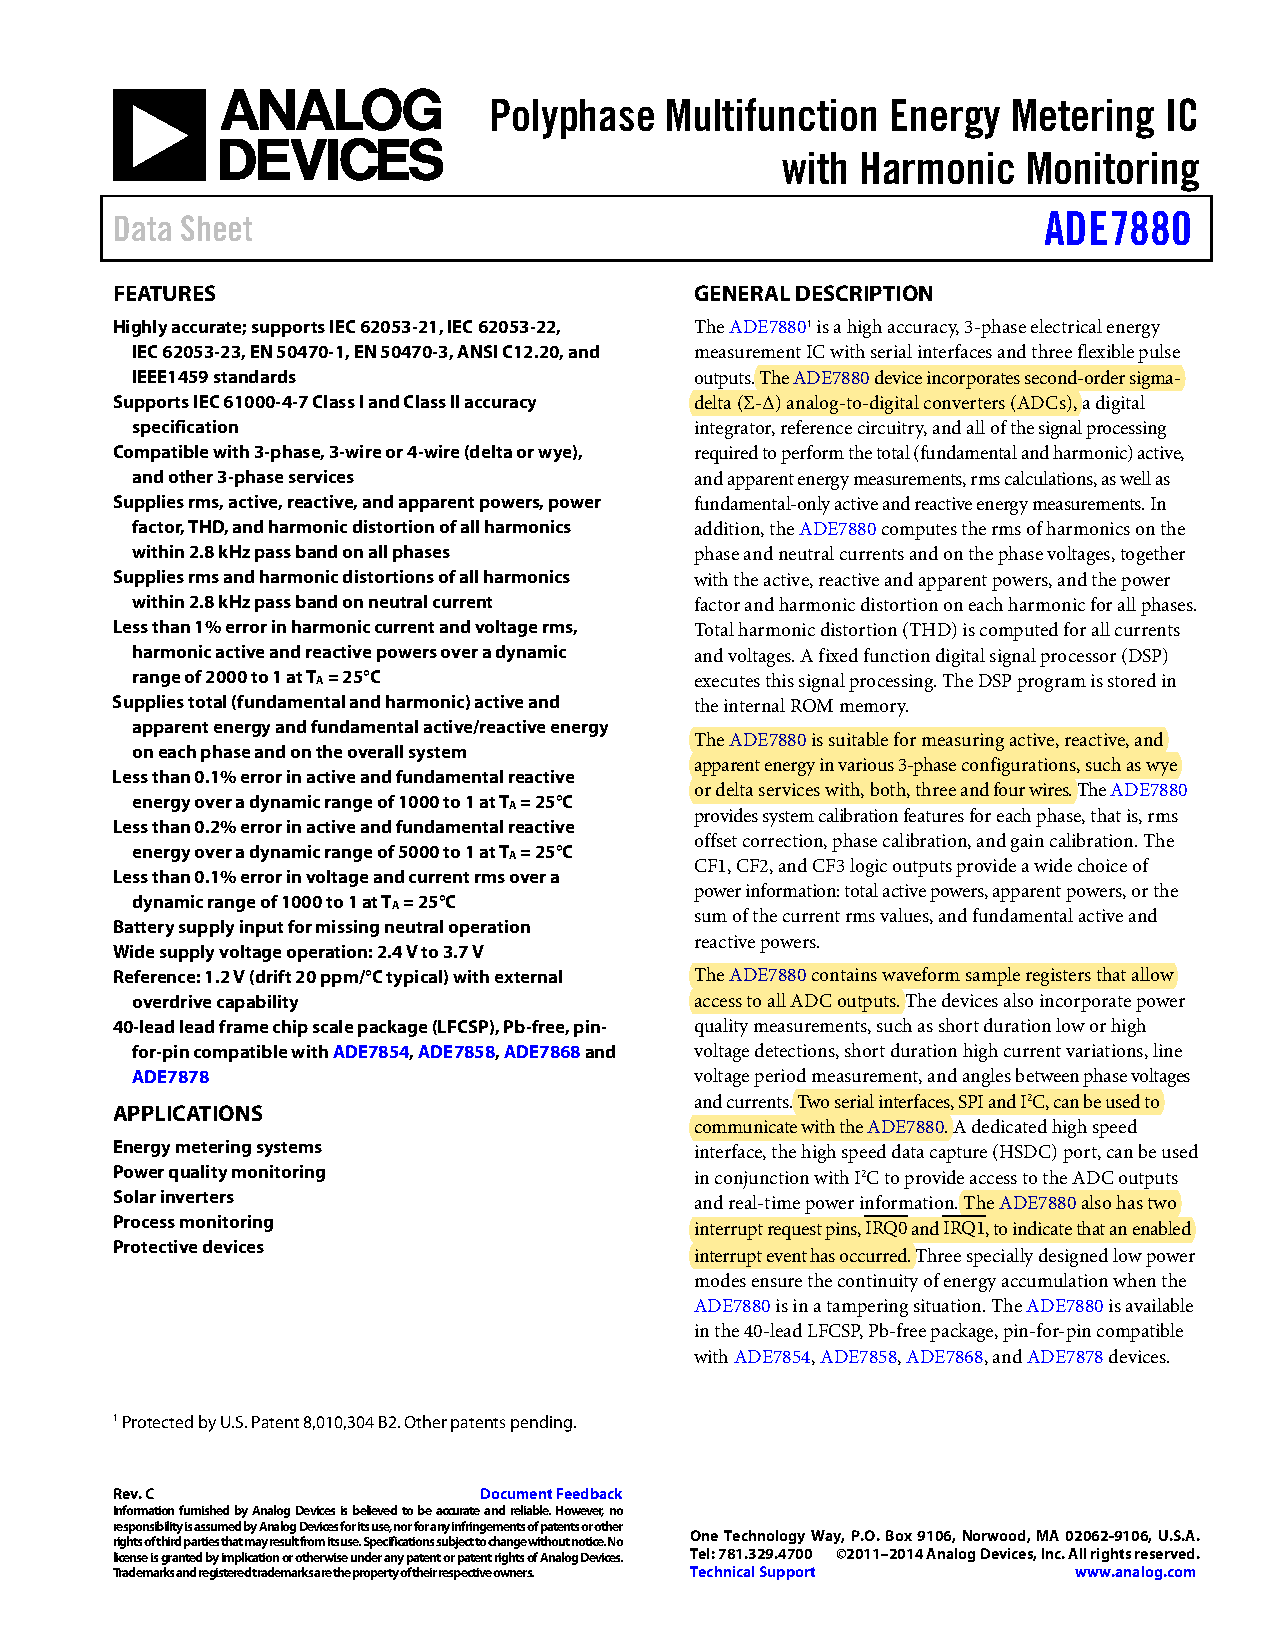
\includepdf[pages = {1,4,5,6,7,8,9,10,12,13,19,23,24,66,76,77,78,79,80,81,82,87,88,89,90,91,92,93,94,95,96,97,98,99,100,101,102,103,104,105,106}]{Material de Consulta/ADE7880}

	\backmatter%@sglvgdor
\end{document}